\documentclass[11pt]{article}
\usepackage[top=1.00in, bottom=1.0in, left=1in, right=1in]{geometry}
\renewcommand{\baselinestretch}{1.1}
\usepackage{graphicx}
\usepackage{natbib}
\usepackage{amsmath}
\usepackage{gensymb}
\usepackage{parskip}
\usepackage{xcolor}
\usepackage{lineno}
\usepackage[normalem]{ulem}

\def\labelitemi{--}
\parindent=0pt

\begin{document}
\renewcommand{\refname}{\CHead{}}

% This has the comments mostly removed and BBL embedded ... otherwise it should be the same as chillingms.tex ...
% though I have not tried compiling it to make sure it is okay (e.g., that I did not accidentally delete stuff!).

\title{The problem and promise of \\ modeling plant leafout under warmer winters} 
\author{E.M. Wolkovich$^{1*}$, Justin Ngo$^1$, Victor Van der Meersch$^1$, Robert D. Guy$^1$ \\ \& Jonathan Auerbach$^2$} 
\maketitle

\emph{Running title:} The problem with chilling

$^1$ Forest \& Conservation Sciences, Faculty of Forestry \& Environmental Stewardship, University of British Columbia, 2424 Main Mall, Vancouver, BC V6T 1Z4, Canada\\
$^2$ Department of Statistics, George Mason University, 4511 Patriot Circle, Fairfax, VA 22030, United States\\
$^*$ e.wolkovich@ubc.ca

\newpage
\linenumbers
\begin{abstract} 
How warmer winters affect plant leafout has major implications for carbon storage and ecosystem stability. Recent evidence that the advance of spring budburst has slowed with anthropogenic climate change has reignited a decades-old debate over winter chilling---the concept that woody temperate plants require sufficient winter cool temperatures to budburst each spring. The problem with chilling is that it does not correspond with an observable event.  This makes models of it rarely falsifiable and of limited use for advancing scientific understanding. In this paper, we review how current research built on the concept of chilling combined with limited data has led to the proliferation of untestable models that are consistent with a wide range of forecasts and provide little insight into actual plant biology. We argue that the concept of chilling should be reevaluated like past theoretical constructs of limited scientific value (such as `dormin' or  `anthesin') to help accelerate our understanding of plant development. This can be done by leveraging new insights on the biochemistry and physiology of dormancy to build better models that fit to both experimental and observational data, and by designing better experiments to more rigorously test theory. 
\end{abstract}


\emph{Keywords:} Chilling, spring phenology, dormancy, endodormancy, process-based modeling, forests
% Data from Walde: https://datadryad.org/dataset/doi:10.5061/dryad.x95x69pnp

\newpage
Plant leafout in the spring has shifted weeks earlier in many regions due to warming from anthropogenic climate change with consequences for a wide range of ecosystem services \citep{keenan2014net,ipcc2022}. Which underlying processes drive this trend, however, is debated, as recent research suggests winter warming may slow or stall further advances \citep{fu2015,piao2017}. Such reports focus on a two-step model of leafout where plants first require cool winter temperatures, often called `chilling,' before they can accumulate enough warm temperatures---`forcing'---to leafout each year (Figure \ref{fig:chillbasics}). This model of chilling is only one of many models proposed since the concept was first introduced \citep[][]{basler2016evaluating,hufkens2018integrated}. But, while forcing ends in an observable event such as leafout, the day plants achieve their chilling requirements coincides with no known measurable event. 

Current models of chilling predict wildly different leafout times for the same study system and temperature regime \citep{guy2014,chuine2016}. 
Even simple models yield radically different predictions for the exact same conditions depending on the choice of parameterization (Figure \ref{fig:nonidentifyme}). Such extreme variability of spring phenology predicted from current models highlights fundamental gaps in our understanding. While decades of experimental evidence suggest that winter temperatures impact leafout \citep{charrier2015,baum2021} new research has highlighted major flaws in current models, including multiple papers now suggesting estimates of `chilling' could easily be artifacts of poor models or correlated observational climate data \citep{decsens,gao2024}. 

Now appears an opportune time to address the problems in our concept of chilling in models of leafout. Because accurate forecasts of spring phenology are critical for carbon sequestration \citep{green2022limits,keenan2014net}, many crops and a number of other services important to humans, there is widespread interest in improving chilling models \citep{Luedeling2015Acta,chuine2016}. At the same time, recent results from molecular and cellular studies of dormancy are providing insights into when and how chilling works \citep{pan2023epigenetic,zhu2021cold}, which could rule in---or out---some of the myriad current models. 
Here, we review the theory of chilling, its origins and potential problems, as well as new opportunities for major advances and how shifting current practices could accelerate progress. We argue that revisiting the current concept of chilling---and its utility---could help build better models and design better experiments. 

\section*{What is chilling?}
How plants in temperature-limited systems avoid leafout during warm spells in the winter has long been debated by plant biologists \citep[e.g.,][]{lamb1948effect,weinberger}. Most work to date has focused on the idea that plants enter some form of dormancy in the fall, which is then released before warm temperatures in the spring begin. This idea hypothesizes that the slow accumulation of cool temperatures---or chilling---over the winter extends through periods of short warm spells in the winter and thus prevents leafout before spring. 

The term `chilling' is now used across numerous fields in plant biology to refer to a process where dormant embryonic tissues exposed to cool temperatures accelerate a life history event that later occurs after warm temperatures (Fig. \ref{fig:chillbasics}). Today the term is most often used for dormant buds that later transition to leafout or flowering, but also used for seeds \citep[though `cold stratification,' which indicates an additional requirement of moist conditions, is more often used for seeds,][]{baskin2000seeds,considine2016language}. While we also focus on chilling in regards to bud dormancy, the mechanisms underlying chilling requirements of seeds likely provide important parallels to bud dormancy, as evolution is more likely to co-opt an existing mechanism than to start from scratch.  
Much of our fundamental understanding of chilling for buds comes from studies on temperate woody fruit crops where chilling can be critical to yield. Peach trees planted into warmer climates well outside their range often have extremely low fruitset because most flower buds do not burst \citep{weinberger,overcash1955effects,erez1971improved}. Early studies of this phenomenon with related experiments---where cut ends of dormant branches (cuttings) exposed to cooler temperatures in chambers burst more fully and more quickly---underlie most of the models of chilling used today for crops and wild tree species \citep[][]{weinberger,ospreebbms}. 

Focused on how chilling can accelerate observable events, researchers have calculated how much `chilling' is required for leafout of forest trees from cutting experiments similar to those used for peaches \citep[reviewed in][]{ospreebbms}, ground observations of budburst \citep{Luedeling2009}, and satellite measures of greenup \citep{kaduk2011predicting}. These estimates rely on phenological models that have become critical across a suite of fields, from climatology, where modeling how vegetation on the land surface responds to anthropogenic climate change affects carbon storage, to crop biology, where `chill units'  guide growers in which specific cultivar to plant and has led to the cross-disciplinary field of phenology \citep{Schwartz:1994he,Cleland:2007or,pmp}. 

Alongside these more macro-scale studies of chilling, molecular approaches have also examined chilling. Many studies have focused on vernalization---cool temperatures required for flowering \citep{kim2009vernalization}---with much work on the herbaceous species \emph{Arabidopsis thaliana}. In woody species, most work has examined chilling before budbreak \citep[][]{azeez2021early,cai2024molecular}. These studies generally use controlled temperatures to vary the hypothesized amount of chilling, and then examine molecular and cellular responses \citep[e.g.,][and see Fig. \ref{fig:modelsketch}]{pan2021aba,azeez2021early,cai2024molecular}.

Today these studies have led to over 30 basic models where accumulated chilling releases plants from dormancy \citep[][]{basler2016evaluating,hufkens2018integrated}. Though early debates considered whether plants were truly dormant or only growing slow \citep[`dormancy' or `rest' versus `quiescence';][]{considine2016language}, today most research assumes a model with two phases of dormancy: (1) endodormany, the period when chilling occurs, and (2) a period between endodormancy but before the observed event, called  ecodormancy (Figure \ref{fig:modelsketch}).  In most models, chilling only accumulates under certain temperatures---traditionally above zero but below 10\degree C---with certain temperatures 
being optimal for the most rapid accumulation of `chill units,' where some unknown sum of chill units breaks endodormancy. Which temperatures are most effective at providing chilling is a common question addressed in experiments, with different experiments providing different answers \citep{vitasselev,baum2021}. 

Variation in responses to chilling across and within species yields hundreds of variants of the basic models \citep[][]{basler2016evaluating,hufkens2018integrated}. Complexity comes from the hypothesized diversity of chilling temperature thresholds and sums across species and populations. Most assume different species require different sums of chill units, and may have different lower, upper, and optimal chill temperatures. Within species, populations may require different sums of chill units, with populations in more mild climates---where warm interruptions in the winter are more common---requiring more chill units than those in areas with cold winters, where temperatures rarely rise above zero before spring \citep{campbell1979,leinonen1996dependence}.  


\section*{The problem with chilling}

\subsection*{An unobserved process}

Chilling is a latent, unobserved process. Typically, 
`chilling' describes the physiological phase (endodormancy) in which a plant experiences environmental temperatures that induce progress towards the next physiological phase (ecodormancy) that ends in budburst (Figure \ref{fig:chillbasics}). The problem is that the transition from endo- to ecodormancy currently corresponds with no clearly measurable phenomenon, and thus the properties of each period cannot be determined from the observed budburst, even under experimental conditions in which the temperature can be manipulated. 

The parameters of a model matching this hypothesized dormancy process are said to be underdetermined or unidentified. For example, consider a simple model in which one would need to estimate the minimum and maximum temperatures that allow chilling to accumulate (two parameters) and the total sum of those temperature units needed to trigger a shift into the next physiological phase (often called `endodormancy break') for one additional parameter. Models then need to estimate when plants start and stop accumulating (two more parameters). An experiment that raises temperatures and observes an earlier leafout could be explained by more rapid chilling accumulation leading to earlier endodormancy break, more rapid ecodormancy break, or an almost limitless mix of the two (Figures \ref{fig:chillbasics}-\ref{fig:nonidentifyme}). 

To address this, models often assign the start date of endodormancy as known (e.g., starting 1 September in the northern hemisphere) and rely on assumptions to set the end date (Figure \ref{fig:nonidentifyme}). A common and widely-used assumption, developed by early work on peaches, is that high and rapid budburst (leaf or flower) is evidence that chilling has been met \citep[i.e. endodormancy has ended,][see also Figure \ref{fig:chillbasics}]{erez1971}, but this assumption has rarely been evaluated for other taxa or populations. The approach of assigning some unknown parameters as known has the benefit of avoiding adding more unknown model parameters, but has led researchers to be overly confident in a model of chilling where more is actually unobserved and unknown than acknowledged. 

\subsection*{Hidden assumptions in complicated models}

% Hidden assumptions and numerous parameters can easily drive diverging models. 
More complex models may seem to solve the identification problem, but often come with their own untestable assumptions. Even if we assume that high and rapid percent budburst signals sufficient chilling, most models today include parameters that cannot be uniquely identified with current data, which explains how one model can often predict a wide variety of leafout possibilities (Figure \ref{fig:nonidentifyme}). The current tacit approach to these major issues likely has contributed to the expansion of models over the last few decades without any clear advances. While various models have added complexity via the shape of the optimal temperature range for chilling, allowing accumulated chilling to be reduced, shifting the start date of chilling, and/or allowing chilling and forcing to act simultaneously \citep{lued2009,gusewell2017,hanninen1990modelling,Kramer1994}, none of these have swept through the field. 

As experiments and models have become more complicated, data have remained relatively uninformative to try to estimate all the complexities the models include. Further, recent models have often relied on even less data \citep{hanninen2019experiments}. Many current methods use only observational data of the timing of leafout (or flowering) to attempt to estimate a model of chilling for different species or locations and project it forward to understand effects of anthropogenic climate change \citep{lued2011,luedeling2012chilling,gao2024}. Perhaps not surprisingly then, which model is deemed best varies strongly by method and approach \citep{Caffarra:2011qf,basler2016evaluating,hufkens2018integrated}, with no clear pattern. 

\subsection*{Unclear aims: Prediction versus mechanistic understanding}

The flood of current models of budburst with similar levels of predictive accuracy is not necessarily a problem, depending on the aim. Many models of chilling are used to guide crop and tree planting---preventing planting too far outside the range of climates with sufficient chilling for a species, population, or cultivar. For this aim, models need to translate climate into relevant chilling and forcing values and define appropriate thresholds, but how exactly each model defines chilling and forcing is immaterial if the predictions are accurate enough (many models of `chill units' are thus based simply on average winter conditions). In such cases moving towards machine learning models---which emphasize predictive accuracy often through black box approaches---may provide more practical models that also clearly acknowledge that the underlying process is obscure \citep{khodadadzadeh}. 

In contrast, if the aim is biological understanding, then the number of highly contrasting but similarly predictive models suggests a problem with the current approach. Models to help elucidate the process that underlies the concept of chilling should represent the current biological understanding. Thus the specification of the model---what parameters it includes, and how well they can be estimated from the data---becomes more important, as does how to evaluate models. Tests that compare models for how accurate they represent our understanding of plant biology, and not only their predictive accuracies across a range of climate regimes, should guide model development. For this aim, new models are unlikely to be enough without new data and approaches that target the major problems facing models of chilling.


\section*{Overcoming the chilling problem}

Richer, more informative data from molecular biology studies and other approaches \citep{fouche2023transport,walde2024stable} hold the promise to elevate chilling from an unobserved complex process to something we understand and can robustly forecast. Taking full advantage of this opportunity, however, would benefit from re-examining the concept of chilling across different disciplines to combine observational and experimental evidence, while providing the opportunity to question the future utility of chilling.

\subsection*{Leverage new molecular insights to overcome problems in the simplest models}

New molecular research provides hope that the transition from endo- to ecodormancy is measurable. Molecular insights have long contributed to crop and forest tree models of chilling \citep{chuinearees}. Decades of work on vernalization have outlined the pathways---and genes---that lead to flowering only after winter's cool temperatures in biennial (herbaceous) populations of \emph{Arabidopsis thaliana} \citep[Figure \ref{fig:modelsketch},][]{Wilczek:2009oa,kim2009vernalization}. Research has linked some of these pathways to similar ones in woody species and have also highlighted the polysaccharide callose (1,3-$\beta$-{\sc D}-glucan) as potentially pivotal for chilling \citep{vanderschoot2014,pan2021aba}. 

Multiple studies across multiple species have now shown that (1) lower temperatures appear to degrade callose and (2) the release/loss of callose appears to re-start cell-to-cell communication before budburst \citep{vanderschoot2014,pandey2026variable}. Taken together, these results suggest the loss of callose may be an indicator of endodormancy release, though other factors, such as  phytohormones, also often change at the same time \citep[][]{rinne2018,tylewicz2018photoperiodic,pan2021aba,andre2022populus}. Whether any of these provide a reliable and easy-to-measure indicator of dormancy release, however, is still unclear (see supplement, `The search for better indicators').

If callose is a major controller of endodormancy and its release, chilling models could be limited to those that match the idea of callose degradation---meaning models that include a temperature range over which the enzyme(s) degrading callose is active (Figure \ref{fig:modelsketch}). In contrast, models using simple temperature thresholds (e.g., all hours below -5\degree C equally allow chilling) would appear less biologically accurate, as enzymes generally do not work over such a wide range of temperatures. 

Other recent insights similarly suggest that such simplified temperature metrics used in many chilling models may not map to molecular realities. For example, new work on how slow growth itself may act  a `long-term thermosensor' \citep{zhao2020temperature} 
adds to an increasing number of molecular studies that suggest plants integrate long-term thermo-sensing in the winter alongside responses to short-term temperatures \citep{antoniou2021feeling,Satake2022}. The best models of leafout may thus need to integrate across multiple timescales. While this could easily complicate models already burdened with complexity, insights from molecular biology could rule out models by focusing on new experiments and modeling approaches. 

\subsection*{Model experimental and observational data together to test assumptions} 
Research on chilling could accelerate by working across what today are three fairly separated silos: 1) model building for crops and other forecasting needs (usually called process-based models), 2) experiments at the branch or whole-plant level, and 3) molecular research. Currently, crop biologists, phenological process-based modelers of forest trees, molecular biologists, and modelers of related processes (e.g., hardiness) 
all develop unique and rarely compared models of dormancy and budburst \citep[but see][]{kovaleskipreprint}, highlighting a major problem, but also a major opportunity. Synthesizing and benchmarking models---and their underlying biological understanding of chilling---across the many research fields developing chilling models today would help identify models that are equivalent and/or perform especially poorly, and could begin to discard some models.  

Comparing models more directly would hopefully drive new approaches that estimate chilling by fitting experimental and observational data together in one model. This is rarely done, in part because of how differently they may be observed, including the challenging diversity of environmental conditions across these two data types (for example, many experiments apply cold temperatures in the dark and include extreme temperature differences, while in observational data photoperiod shifts each day and temperatures are more similar) but also because of separate modeling approaches. Researchers almost never fit process-based models to new empirical data; instead they use so-called `statistical models' that often follow canonical treatment designs (e.g., ANOVA). Statistical models are usually far simpler, and make a suite of unstated assumptions that contradict the current understanding of chilling 
(see Figure \ref{fig:multimodelexps}). Many of the original studies that led to the concept of chilling, however, bridged across observational and experimental studies more often and leveraged datasets that created greater extremes in observational data---by focusing on crops planted well outside their natural range \citep[e.g., peaches in Florida and Israel, ][]{erez1971,richardson1974}. These approaches did this in part by more explicitly mapping from biological processes to statistical models, making it easier to use the models to define new tests to challenge the biological theory. 

Experiments bridging across methods may have the greatest opportunity to provide data that would truly challenge current models of chilling. Testing models across large environmental gradients in the field is one of the best ways to find out where models work---and where they fail. For example, molecular biologists tested vernalization models by comparing predicted to observed flowering times in a common garden design across Europe \citep[][]{Wilczek:2009oa} and supported the temperature-dependent growth model by testing its predictions of what happens when growth is altered but temperature is held constant \citep{zhao2020temperature}. Similar examples for challenging other models of chilling date back over 40 years to when many of the models used today were developed \citep{richardson1974,chuine2016,ospreebbms}, but could take place now. Models of chilling can make predictions under lower field chilling then test them using individuals planted beyond the range (either by planting those individuals now or identifying such cases in forestry provenance trials or similar). Process-based modelers could also challenge their models through more dramatic variation in biology; new experiments that include genetic mutants or similar variants \citep[e.g.,][]{azeez2021early,pan2023epigenetic} could help test the effects of genes that putatively influence endo/ecodormancy under a spectrum of natural conditions \citep{Satake2022}. 


\subsection*{Is the concept of chilling necessary for scientific progress?}  

Results from new molecular experiments designed to identify novel ways to directly observe and measure chilling could upend the current concept of chilling. As increasing evidence suggests the concept aligns with multiple shifts at the cellular and molecular level (Figure \ref{fig:modelsketch}), researchers across disciplines will need to consider how to continue using the term `chilling.' One approach is to try to align previous and current definitions through new studies, 
for example, by testing for callose loss \citep{yu2024building} alongside previously used markers of dormancy shifts---including the often-used bioassay of high and rapid budburst at higher temperatures (indicating endodormancy release) and additional methods, such as weighing flower buds \citep{chuine2016} or tracing water reactivation into cells \citep{faust1991bound,Kalcsits2009,walde2024stable}. 
Another approach is to work towards new terms that more clearly align with new measurements and insights. 

Because chilling is an unobserved process, it may link eventually to one measurable compound or regulator (similar to florigen or auxin) or to a more complicated biology, making the term less useful \citep{aksenova2006florigen}. Current results suggest the latter, and already the term `chilling' is used to mean different things. For example, while we focus here on the term as an accumulation process during an unobserved physiological phase (endodormancy), many experiments currently use the term `chilling' to refer to a treatment where researchers do not know the physiological phase \citep[for example, cuttings or buds from woody plants are often chilled at 5\degree C for 6 weeks in the dark in a `chilling' treatment, then transferred to warm `forcing' conditions,][]{flynn2018,ospreebbms}.  

Diverging definitions suggest that the best path for chilling may be to follow that of other terms modern plant biologists may not remember, such as dormin or anthesin \citep[hypothesized compounds to induce dormancy and floral anthesis, respectively,][]{aksenova2006florigen,dorffling2015discovery}, and let the term fade into obsolescence. Fundamental research on the physiological and molecular biological mechanisms of bud dormancy is primed to discover new measurable processes and observable events related to what we call `chilling' today. With this, new terms and concepts that better match our improved understanding could emerge to aid research across the disciplines studying chilling. Models for forecasting and new experiments at the branch and whole plant level could focus on predicting and measuring these new events and processes. `Chill units'  for widely planted forest trees and specific varieties of crops, which are already less linked to the mechanism of chilling, would likely hold on longer. They too, however, may shift to new estimates or units based on better measures, especially as increasing anthropogenic climate change makes getting the mechanistic biology of plant development right all the more important. 


\clearpage
\bibliographystyle{/Users/Lizzie/Documents/EndnoteRelated/Bibtex/styles/besjournals}
\section{References}
\begin{thebibliography}{66}
\providecommand{\natexlab}[1]{#1}

\bibitem[{Aksenova \emph{et~al.}(2006)Aksenova, Milyaeva \&
  Romanov}]{aksenova2006florigen}
Aksenova, N., Milyaeva, E. \& Romanov, G. (2006) Florigen goes molecular:
  seventy years of the hormonal theory of flowering regulation. \emph{Russian
  Journal of Plant Physiology} \textbf{53}, 401--406.

\bibitem[{Andr{\'e} \emph{et~al.}(2022)Andr{\'e}, Zambrano, Zhang, Lee,
  R{\"u}hl, Marcon \& Nilsson}]{andre2022populus}
Andr{\'e}, D., Zambrano, J.A., Zhang, B., Lee, K.C., R{\"u}hl, M., Marcon, A.
  \& Nilsson, O. (2022) Populus svl acts in leaves to modulate the timing of
  growth cessation and bud set. \emph{Frontiers in Plant Science} \textbf{13},
  823019.

\bibitem[{Antoniou-Kourounioti \emph{et~al.}(2021)Antoniou-Kourounioti, Zhao,
  Dean \& Howard}]{antoniou2021feeling}
Antoniou-Kourounioti, R.L., Zhao, Y., Dean, C. \& Howard, M. (2021) Feeling
  every bit of winter--distributed temperature sensitivity in vernalization.
  \emph{Frontiers in Plant Science} \textbf{12}, 628726.

\bibitem[{Azeez \emph{et~al.}(2021)Azeez, Zhao, Singh, Yordanov, Dash,
  Miskolczi, Stojkovi{\v{c}}, Strauss, Bhalerao \& Busov}]{azeez2021early}
Azeez, A., Zhao, Y.C., Singh, R.K., Yordanov, Y.S., Dash, M., Miskolczi, P.,
  Stojkovi{\v{c}}, K., Strauss, S.H., Bhalerao, R.P. \& Busov, V.B. (2021)
  Early bud-break 1 and early bud-break 3 control resumption of poplar growth
  after winter dormancy. \emph{Nature communications} \textbf{12}, 1123.

\bibitem[{Baskin \& Baskin(2000)}]{baskin2000seeds}
Baskin, C.C. \& Baskin, J.M. (2000) \emph{Seeds: ecology, biogeography, and,
  evolution of dormancy and germination}. Academic press.

\bibitem[{Basler(2016)}]{basler2016evaluating}
Basler, D. (2016) Evaluating phenological models for the prediction of leaf-out
  dates in six temperate tree species across central europe. \emph{Agricultural
  and Forest Meteorology} \textbf{217}, 10--21.

\bibitem[{Baumgarten \emph{et~al.}(2021)Baumgarten, Zohner, Gessler \&
  Vitasse}]{baum2021}
Baumgarten, F., Zohner, C.M., Gessler, A. \& Vitasse, Y. (2021) Chilled to be
  forced: the best dose to wake up buds from winter dormancy. \emph{New
  Phytologist} \textbf{230}, 1366--1377.

\bibitem[{Caffarra \emph{et~al.}(2011)Caffarra, Donnelly \&
  Chuine}]{Caffarra:2011qf}
Caffarra, A., Donnelly, A. \& Chuine, I. (2011) {Modelling the timing of
  \emph{Betula pubescens} budburst. II. Integrating complex effects of
  photoperiod into process-based models}. \emph{Climate Research} \textbf{46},
  159--170.

\bibitem[{Cai \emph{et~al.}(2024)Cai, Jin, Tian, Huang, Wang, Zhang, Sun \&
  Shao}]{cai2024molecular}
Cai, F., Jin, X., Tian, Y., Huang, Z., Wang, X., Zhang, Y., Sun, Y. \& Shao, C.
  (2024) Molecular regulation of bud dormancy in perennial plants. \emph{Plant
  Growth Regulation} \textbf{102}, 1--11.

\bibitem[{Campbell \& Sugano(1979)}]{campbell1979}
Campbell, R.K. \& Sugano, A.I. (1979) {Genecology of bud-burst phenology in
  Douglas-fir - response to flushing temperature and chilling}. \emph{Botanical
  Gazette} \textbf{140}, 223--231.

\bibitem[{Charrier \emph{et~al.}(2015)Charrier, Ngao, Saudreau \&
  Ameglio}]{charrier2015}
Charrier, G., Ngao, J., Saudreau, M. \& Ameglio, T. (2015) Effects of
  environmental factors and management practices on microclimate, winter
  physiology, and frost resistance in trees. \emph{Frontiers in Plant Science}
  \textbf{6}.

\bibitem[{Chuine \emph{et~al.}(2016)Chuine, Bonhomme, Legave,
  de~Cortazar-Atauri, Charrier, Lacointe \& Ameglio}]{chuine2016}
Chuine, I., Bonhomme, M., Legave, J.M., de~Cortazar-Atauri, I.G., Charrier, G.,
  Lacointe, A. \& Ameglio, T. (2016) Can phenological models predict tree
  phenology accurately in the future? the unrevealed hurdle of endodormancy
  break. \emph{Global Change Biology} \textbf{22}, 3444--3460.

\bibitem[{Chuine \emph{et~al.}(2013)Chuine, Garcia~de Cortazar~Atauri, Hanninen
  \& Kramer}]{pmp}
Chuine, I., Garcia~de Cortazar~Atauri, I., Hanninen, H. \& Kramer, K. (2013)
  \emph{Plant development models}, pp. 275--293. Kluwer, Dordrecht, the
  Netherlands.

\bibitem[{Chuine \& Regniere(2017)}]{chuinearees}
Chuine, I. \& Regniere, J. (2017) Process-based models of phenology for plants
  and animals. \emph{Annual Review of Ecology, Evolution, and Systematics}
  \textbf{48}, 159--182.

\bibitem[{Cleland \emph{et~al.}(2007)Cleland, Chuine, Menzel, Mooney \&
  Schwartz}]{Cleland:2007or}
Cleland, E.E., Chuine, I., Menzel, A., Mooney, H.A. \& Schwartz, M.D. (2007)
  Shifting plant phenology in response to global change. \emph{Trends in
  Ecology \& Evolution} \textbf{22}, 357--365.

\bibitem[{Considine \& Considine(2016)}]{considine2016language}
Considine, M.J. \& Considine, J.A. (2016) On the language and physiology of
  dormancy and quiescence in plants. \emph{Journal of Experimental Botany}
  \textbf{67}, 3189--3203.

\bibitem[{D{\"o}rffling(2015)}]{dorffling2015discovery}
D{\"o}rffling, K. (2015) The discovery of abscisic acid: a retrospect.
  \emph{Journal of Plant Growth Regulation} \textbf{34}, 795--808.

\bibitem[{Erez \& Lavee(1971)}]{erez1971}
Erez, A. \& Lavee, S. (1971) Effect of climatic conditions on dormancy
  development of peach buds. i. temperature. \emph{Journal of the American
  Society for Horticultural Science} .

\bibitem[{Erez \emph{et~al.}(1971)Erez, Lavee \& Samish}]{erez1971improved}
Erez, A., Lavee, S. \& Samish, R.M. (1971) Improved methods for breaking rest
  in the peach and other deciduous fruit species. .

\bibitem[{Ettinger \emph{et~al.}(2020)Ettinger, Chamberlain, Morales-Castilla,
  Buonaiuto, Flynn, Savas, Samaha \& Wolkovich}]{ospreebbms}
Ettinger, A.K., Chamberlain, C.J., Morales-Castilla, I., Buonaiuto, D.M.,
  Flynn, D.F.B., Savas, T., Samaha, J.A. \& Wolkovich, E.M. (2020) Winter
  temperatures predominate in spring phenological responses to warming.
  \emph{Nature Climate Change} \textbf{10}, 1137--U119.

\bibitem[{Faust \emph{et~al.}(1991)Faust, Liu, Millard \&
  Stutte}]{faust1991bound}
Faust, M., Liu, D., Millard, M.M. \& Stutte, G. (1991) Bound versus free water
  in dormant apple buds---a theory for endodormancy. \emph{HortScience}
  \textbf{26}, 887--890.

\bibitem[{Flynn \& Wolkovich(2018)}]{flynn2018}
Flynn, D.F.B. \& Wolkovich, E.M. (2018) Temperature and photoperiod drive
  spring phenology across all species in a temperate forest community.
  \emph{New Phytologist} \textbf{29}, 1135--1492.

\bibitem[{Fouch{\'e} \emph{et~al.}(2023)Fouch{\'e}, Bonnet, Bonnet \&
  Wenden}]{fouche2023transport}
Fouch{\'e}, M., Bonnet, H., Bonnet, D.M. \& Wenden, B. (2023) Transport
  capacity is uncoupled with endodormancy breaking in sweet cherry buds:
  physiological and molecular insights. \emph{Frontiers in Plant Science}
  \textbf{14}, 1240642.

\bibitem[{Fu \emph{et~al.}(2015)Fu, Zhao, Piao, Peaucelle, Peng, Zhou, Ciais,
  Huang, Menzel, Uelas, Song, Vitasse, Zeng \& Janssens}]{fu2015}
Fu, Y.S.H., Zhao, H.F., Piao, S.L., Peaucelle, M., Peng, S.S., Zhou, G.Y.,
  Ciais, P., Huang, M.T., Menzel, A., Uelas, J.P., Song, Y., Vitasse, Y., Zeng,
  Z.Z. \& Janssens, I.A. (2015) Declining global warming effects on the
  phenology of spring leaf unfolding. \emph{Nature} \textbf{526}, 104--107.

\bibitem[{Gao \emph{et~al.}(2024)Gao, Richardson, Friedl, Moon \&
  Gray}]{gao2024}
Gao, X., Richardson, A.D., Friedl, M.A., Moon, M. \& Gray, J.M. (2024) Thermal
  forcing versus chilling? misspecification of temperature controls in spring
  phenology models. \emph{Global Ecology and Biogeography} \textbf{33}, e13932.

\bibitem[{Green \& Keenan(2022)}]{green2022limits}
Green, J.K. \& Keenan, T.F. (2022) The limits of forest carbon sequestration.
  \emph{Science} \textbf{376}, 692--693.

\bibitem[{Gusewell \emph{et~al.}(2017)Gusewell, Furrer, Gehrig \&
  Pietragalla}]{gusewell2017}
Gusewell, S., Furrer, R., Gehrig, R. \& Pietragalla, B. (2017) Changes in
  temperature sensitivity of spring phenology with recent climate warming in
  switzerland are related to shifts of the preseason. \emph{Global Change
  Biology} \textbf{23}, 5189--5202.

\bibitem[{Guy(2014)}]{guy2014}
Guy, R.D. (2014) The early bud gets to warm. \emph{New Phytologist}
  \textbf{202}, 7--9.

\bibitem[{H{\"a}nninen(1990)}]{hanninen1990modelling}
H{\"a}nninen, H. (1990) \emph{Modelling bud dormancy release in trees from cool
  and temperate regions.} 213.

\bibitem[{H{\"a}nninen \emph{et~al.}(2019)H{\"a}nninen, Kramer, Tanino, Zhang,
  Wu \& Fu}]{hanninen2019experiments}
H{\"a}nninen, H., Kramer, K., Tanino, K., Zhang, R., Wu, J. \& Fu, Y.H. (2019)
  Experiments are necessary in process-based tree phenology modelling.
  \emph{Trends in Plant Science} \textbf{24}, 199--209.

\bibitem[{Hufkens \emph{et~al.}(2018)Hufkens, Basler, Milliman, Melaas \&
  Richardson}]{hufkens2018integrated}
Hufkens, K., Basler, D., Milliman, T., Melaas, E.K. \& Richardson, A.D. (2018)
  An integrated phenology modelling framework in r. \emph{Methods in Ecology
  and Evolution} \textbf{9}, 1276--1285.

\bibitem[{Kaduk \& Los(2011)}]{kaduk2011predicting}
Kaduk, J.D. \& Los, S.O. (2011) Predicting the time of green up in temperate
  and boreal biomes. \emph{Climatic Change} \textbf{107}, 277--304.

\bibitem[{Kalcsits \emph{et~al.}(2009)Kalcsits, Kendall, Silim \&
  Tanino}]{Kalcsits2009}
Kalcsits, L., Kendall, E., Silim, S. \& Tanino, K. (2009) Magnetic resonance
  microimaging indicates water diffusion correlates with dormancy induction in
  cultured hybrid poplar (populus spp.) buds. \emph{Tree Physiology}
  \textbf{29}, 1269--1277.

\bibitem[{Keenan \emph{et~al.}(2014)Keenan, Gray, Friedl, Toomey, Bohrer,
  Hollinger, Munger, O'Keefe, Schmid, Wing \emph{et~al.}}]{keenan2014net}
Keenan, T.F., Gray, J., Friedl, M.A., Toomey, M., Bohrer, G., Hollinger, D.Y.,
  Munger, J.W., O'Keefe, J., Schmid, H.P., Wing, I.S. \emph{et~al.} (2014) Net
  carbon uptake has increased through warming-induced changes in temperate
  forest phenology. \emph{Nature Climate Change} \textbf{4}, 598--604.

\bibitem[{Khodadadzadeh \emph{et~al.}(2024)Khodadadzadeh, Kalverla \&
  Zurita-Milla}]{khodadadzadeh}
Khodadadzadeh, M., Kalverla, P. \& Zurita-Milla, R. (2024) Harmonizing machine
  learning based phenological modeling: A unified workflow for comparative
  analyses. \emph{IGARSS 2024 - 2024 IEEE International Geoscience and Remote
  Sensing Symposium}, pp. 5333--5336.

\bibitem[{Kim \emph{et~al.}(2009)Kim, Doyle, Sung \&
  Amasino}]{kim2009vernalization}
Kim, D.H., Doyle, M.R., Sung, S. \& Amasino, R.M. (2009) Vernalization: winter
  and the timing of flowering in plants. \emph{Annual Review of Cell and
  Developmental} \textbf{25}, 277--299.

\bibitem[{Kovaleski(2022)}]{kovaleskipreprint}
Kovaleski, A. (2022) Woody species do not differ in dormancy progression:
  differences in time to budbreak due to forcing and cold hardiness.
  \emph{Proceedings of the National Academy of Sciences} \textbf{119},
  e2112250119.

\bibitem[{Kramer({1994})}]{Kramer1994}
Kramer, K. ({1994}) {Selelecting a model to predict the onset of growth of
  \emph{Fagus sylvatica}}. \emph{Journal of Applied Ecology} \textbf{{31}},
  {172--181}.

\bibitem[{Lamb(1948)}]{lamb1948effect}
Lamb, R.C. (1948) {Effect of temperatures above and below freezing on the
  breaking of rest in the Latham raspberry}. \emph{{Proceedings of the American
  Society for Horticultural Science}} \textbf{51}, 313--315.

\bibitem[{Leinonen(1996)}]{leinonen1996dependence}
Leinonen, I. (1996) Dependence of dormancy release on temperature in different
  origins of pinus sylvestris and betula pendula seedlings. \emph{Scandinavian
  Journal of Forest Research} \textbf{11}, 122--128.

\bibitem[{Luedeling \emph{et~al.}(2012)Luedeling, Blanke \&
  Gebauer}]{luedeling2012chilling}
Luedeling, E., Blanke, M. \& Gebauer, J. (2012) Chilling challenges in a
  warming world. \emph{II International Symposium on Horticulture in Europe
  1099}, pp. 901--907.

\bibitem[{Luedeling \emph{et~al.}(2015)Luedeling, Blanke \&
  Gebauer}]{Luedeling2015Acta}
Luedeling, E., Blanke, M. \& Gebauer, J. (2015) \emph{Chilling Challenges in a
  Warming World}, vol. 1099 of \emph{Acta Horticulturae}, pp. 901--907.

\bibitem[{Luedeling \emph{et~al.}(2011)Luedeling, Girvetz, Semenov \&
  Brown}]{lued2011}
Luedeling, E., Girvetz, E.H., Semenov, M.A. \& Brown, P.H. (2011) Climate
  change affects winter chill for temperate fruit and nut trees. \emph{Plos
  One} \textbf{6}.

\bibitem[{Luedeling \emph{et~al.}(2009{\natexlab{a}})Luedeling, Zhang \&
  Girvetz}]{lued2009}
Luedeling, E., Zhang, M.H. \& Girvetz, E.H. (2009{\natexlab{a}}) {Climatic
  changes lead to declining winter chill for fruit and nut trees in California
  during 1950-2099}. \emph{Plos One} \textbf{4}.

\bibitem[{Luedeling \emph{et~al.}(2009{\natexlab{b}})Luedeling, Zhang,
  McGranahan \& Leslie}]{Luedeling2009}
Luedeling, E., Zhang, M.H., McGranahan, G. \& Leslie, C. (2009{\natexlab{b}})
  Validation of winter chill models using historic records of walnut phenology.
  \emph{Agricultural and Forest Meteorology} \textbf{149}, 1854--1864.

\bibitem[{Overcash \& Campbell(1955)}]{overcash1955effects}
Overcash, J. \& Campbell, J. (1955) The effects of intermittent warm and cold
  periods on breaking the rest period of peach leaf buds. .

\bibitem[{Pan \emph{et~al.}(2023)Pan, Li, Du, Zhao, Xin, Wang, Liu, Lin, Fang,
  Yang \emph{et~al.}}]{pan2023epigenetic}
Pan, W., Li, J., Du, Y., Zhao, Y., Xin, Y., Wang, S., Liu, C., Lin, Z., Fang,
  S., Yang, Y. \emph{et~al.} (2023) {Epigenetic silencing of callose synthase
  by VIL1 promotes bud-growth transition in lily bulbs}. \emph{Nature Plants}
  \textbf{9}, 1451--1467.

\bibitem[{Pan \emph{et~al.}(2021)Pan, Liang, Sui, Li, Liu, Xin, Zhang, Wang,
  Zhao, Zhang \emph{et~al.}}]{pan2021aba}
Pan, W., Liang, J., Sui, J., Li, J., Liu, C., Xin, Y., Zhang, Y., Wang, S.,
  Zhao, Y., Zhang, J. \emph{et~al.} (2021) {ABA and bud dormancy in perennials:
  current knowledge and future perspective}. \emph{Genes} \textbf{12}, 1635.

\bibitem[{Pandey \emph{et~al.}(2026)Pandey, Moraes, Nair, Aryal, Azeez,
  Miskolczi, Maucort, Cordeli{\`e}res, Brocard, Davis
  \emph{et~al.}}]{pandey2026variable}
Pandey, S.K., Moraes, T.S., Nair, A., Aryal, B., Azeez, A., Miskolczi, P.,
  Maucort, G., Cordeli{\`e}res, F.P., Brocard, L., Davis, G.V. \emph{et~al.}
  (2026) Variable temperature processing by plasmodesmata regulates robust bud
  dormancy release. \emph{Nature Communications} \textbf{17}, 348.

\bibitem[{Piao \emph{et~al.}(2017)Piao, Liu, Wang, Peng, Ciais, Huang,
  Ahlstrom, Burkhart, Chevallier, Janssens, Jeong, Lin, Mao, Miller, Mohammat,
  Myneni, Penuelas, Shi, Stohl, Yao, Zhu \& Tans}]{piao2017}
Piao, S.L., Liu, Z., Wang, T., Peng, S.S., Ciais, P., Huang, M.T., Ahlstrom,
  A., Burkhart, J.F., Chevallier, F., Janssens, I.A., Jeong, S.J., Lin, X.,
  Mao, J.F., Miller, J., Mohammat, A., Myneni, R.B., Penuelas, J., Shi, X.Y.,
  Stohl, A., Yao, Y.T., Zhu, Z.C. \& Tans, P.P. (2017) Weakening temperature
  control on the interannual variations of spring carbon uptake across northern
  lands. \emph{Nature Climate Change} \textbf{7}, 359--+.

\bibitem[{P{\"o}rtner \emph{et~al.}(2022)P{\"o}rtner, Roberts, Tignor,
  Poloczanska, Mintenbeck, Alegr{\'\i}a, Craig, Langsdorf, L{\"o}schke,
  M{\"o}ller, Okem \& Rama}]{ipcc2022}
P{\"o}rtner, H.O., Roberts, D.C., Tignor, M., Poloczanska, E.S., Mintenbeck,
  K., Alegr{\'\i}a, A., Craig, M., Langsdorf, S., L{\"o}schke, S., M{\"o}ller,
  V., Okem, A. \& Rama, B. (2022) \emph{Climate Change 2022: Impacts,
  Adaptation and Vulnerability. Contribution of Working Group II to the Sixth
  Assessment Report of the Intergovernmental Panel on Climate Change}.
  Cambridge University Press.

\bibitem[{Richardson(1974)}]{richardson1974}
Richardson, E. (1974) A model for estimating the completion of rest for
  {`Redhaven' and 'Elberta'} peach trees. \emph{HortScience} \textbf{9},
  331--332.

\bibitem[{Rinne \emph{et~al.}(2018)Rinne, Paul \& van~der Schoot}]{rinne2018}
Rinne, P.L.H., Paul, L.K. \& van~der Schoot, C. (2018) Decoupling photo- and
  thermoperiod by projected climate change perturbs bud development, dormancy
  establishment and vernalization in the model tree populus. \emph{BMC Plant
  Biology} \textbf{18}.

\bibitem[{Satake \emph{et~al.}(2022)Satake, Nagahama \& Sasaki}]{Satake2022}
Satake, A., Nagahama, A. \& Sasaki, E. (2022) A cross-scale approach to unravel
  the molecular basis of plant phenology in temperate and tropical climates.
  \emph{New Phytologist} \textbf{233}, 2340--2353.

\bibitem[{Schwartz(1994)}]{Schwartz:1994he}
Schwartz, M.D. (1994) Monitoring global change with phenology -- the case of
  the spring green wave. \emph{International Journal of Biometeorology}
  \textbf{38}, 18--22.

\bibitem[{Tylewicz \emph{et~al.}(2018)Tylewicz, Petterle, Marttila, Miskolczi,
  Azeez, Singh, Immanen, M{\"a}hler, Hvidsten, Eklund
  \emph{et~al.}}]{tylewicz2018photoperiodic}
Tylewicz, S., Petterle, A., Marttila, S., Miskolczi, P., Azeez, A., Singh,
  R.K., Immanen, J., M{\"a}hler, N., Hvidsten, T.R., Eklund, D.M. \emph{et~al.}
  (2018) Photoperiodic control of seasonal growth is mediated by aba acting on
  cell-cell communication. \emph{Science} \textbf{360}, 212--215.

\bibitem[{van~der Schoot \emph{et~al.}(2014)van~der Schoot, Paul \&
  Rinne}]{vanderschoot2014}
van~der Schoot, C., Paul, L.K. \& Rinne, P.L.H. (2014) The embryonic shoot: a
  lifeline through winter. \emph{Journal of Experimental Botany} \textbf{65},
  1699--1712.

\bibitem[{Vitasse \emph{et~al.}(2013)Vitasse, Hoch, Randin, Lenz, Kollas,
  Scheepens \& Koerner}]{vitasselev}
Vitasse, Y., Hoch, G., Randin, C.F., Lenz, A., Kollas, C., Scheepens, J.F. \&
  Koerner, C. (2013) Elevational adaptation and plasticity in seedling
  phenology of temperate deciduous tree species. \emph{Oecologia} \textbf{171},
  663--678.

\bibitem[{Walde \emph{et~al.}(2024)Walde, Wenden, Chuine, Gessler, Saurer \&
  Vitasse}]{walde2024stable}
Walde, M.G., Wenden, B., Chuine, I., Gessler, A., Saurer, M. \& Vitasse, Y.
  (2024) Stable water isotopes reveal the onset of bud dormancy in temperate
  trees, whereas water content is a better proxy for dormancy release.
  \emph{Tree Physiology} \textbf{44}, tpae028.

\bibitem[{Walde \emph{et~al.}(2022)Walde, Wu, Fox, Baumgarten, Fu, Wang \&
  Vitasse}]{walde2022higher}
Walde, M.G., Wu, Z., Fox, T., Baumgarten, F., Fu, Y.H., Wang, S. \& Vitasse, Y.
  (2022) Higher spring phenological sensitivity to forcing temperatures of
  asian compared to european tree species under low and high pre-chilling
  conditions. \emph{Frontiers in Forests and Global Change} \textbf{5},
  1063127.

\bibitem[{Weinberger(1950)}]{weinberger}
Weinberger, J.H. (1950) Chilling requirements of peach varieties.
  \emph{Proceedings of the American Society for Horticultural Science}
  \textbf{56}, 122--128.

\bibitem[{Wilczek \emph{et~al.}(2009)Wilczek, Roe, Knapp, Cooper,
  Lopez-Gallego, Martin, Muir, Sim, Walker, Anderson, Egan, Moyers, Petipas,
  Giakountis, Charbit, Coupland, Welch \& Schmitt}]{Wilczek:2009oa}
Wilczek, A.M., Roe, J.L., Knapp, M.C., Cooper, M.D., Lopez-Gallego, C., Martin,
  L.J., Muir, C.D., Sim, S., Walker, A., Anderson, J., Egan, J.F., Moyers,
  B.T., Petipas, R., Giakountis, A., Charbit, E., Coupland, G., Welch, S.M. \&
  Schmitt, J. (2009) Effects of genetic perturbation on seasonal life history
  plasticity. \emph{Science} \textbf{323}, 930--934.

\bibitem[{Wolkovich \emph{et~al.}(2021)Wolkovich, Auerbach, Chamberlain,
  Buonaiuto, Ettinger, Morales-Castilla \& Gelman}]{decsens}
Wolkovich, E.M., Auerbach, J., Chamberlain, C.J., Buonaiuto, D.M., Ettinger,
  A.K., Morales-Castilla, I. \& Gelman, A. (2021) A simple explanation for
  declining temperature sensitivity with warming. \emph{Global Change Biology}
  \textbf{27}, 4947--4949.

\bibitem[{Yu \emph{et~al.}(2024)Yu, Wenden, Ferguson \& Tian}]{yu2024building}
Yu, S., Wenden, B., Ferguson, L. \& Tian, L. (2024) Building climate resilient
  deciduous tree crops by deciphering winter dormancy.

\bibitem[{Zhao \emph{et~al.}(2020)Zhao, Antoniou-Kourounioti, Calder, Dean \&
  Howard}]{zhao2020temperature}
Zhao, Y., Antoniou-Kourounioti, R.L., Calder, G., Dean, C. \& Howard, M. (2020)
  Temperature-dependent growth contributes to long-term cold sensing.
  \emph{Nature} \textbf{583}, 825--829.

\bibitem[{Zhu \emph{et~al.}(2021)Zhu, Lister \& Dean}]{zhu2021cold}
Zhu, P., Lister, C. \& Dean, C. (2021) Cold-induced arabidopsis frigida nuclear
  condensates for flc repression. \emph{Nature} \textbf{599}, 657--661.

\end{thebibliography}


\clearpage
\section{Figures}

\begin{figure}[h!]
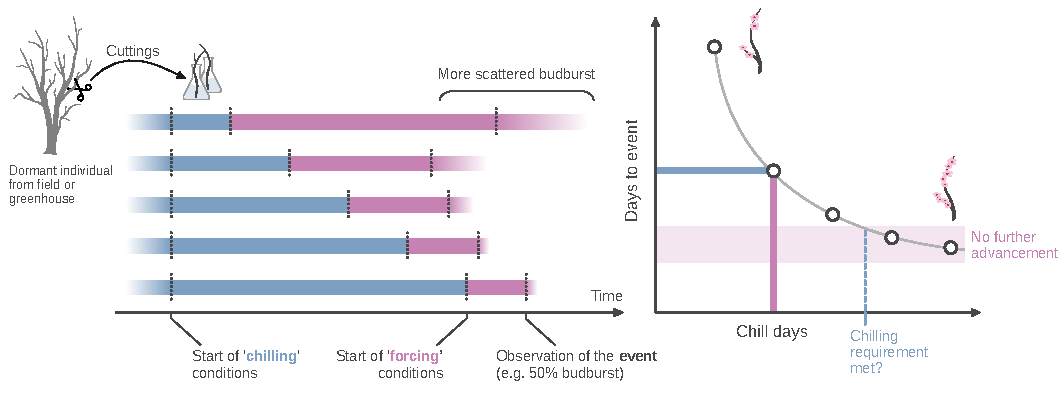
\includegraphics[width=1\textwidth]{..//figures/chillbasic/chillBasic_flowers.pdf}
\caption{
The term chilling generally refers to a process where dormant embryonic tissues exposed to cool temperatures accelerate a plant event that later occurs. While chilling cannot be directly observed currently, experiments for over a hundred years have tried to identify how much chilling plants need by finding the conditions that lead to rapid and full budburst (see right side where chilling is shown as the modeled unit of `chill days'). Many studies have measured this via experiments that take dormant tissue (e.g., cut ends of tree branches taken from the field during the winter), which they then expose to sequential cool temperature treatments (generally called `chilling' treatments or conditions) followed by warmer temperature treatments (called `forcing' treatments or conditions), and observe budburst (left). Required chilling is then defined from these experiments by when additional cool temperatures do not yield faster and more complete budburst (right).} % Data in cchillbasic currently from ospreechillthielges75.pdf 
\label{fig:chillbasics}
\end{figure}

\begin{figure}[h!]
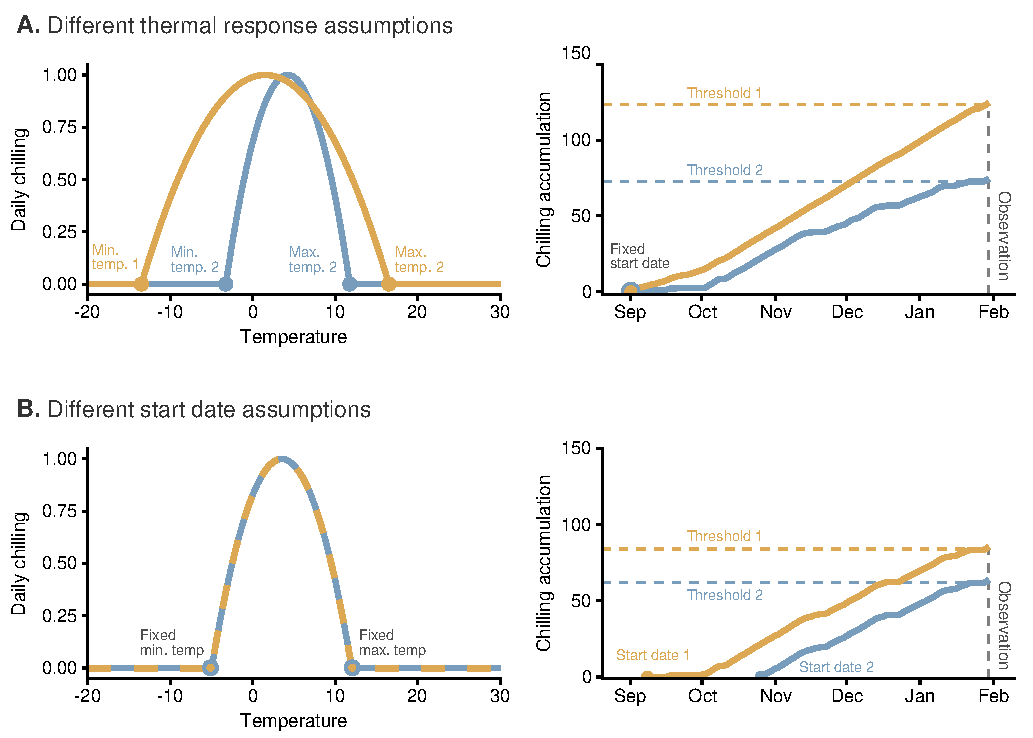
\includegraphics[width=0.8\textwidth]{..//analyses/figures/non_identifiability.pdf}
\caption{\textbf{Current models of chilling cannot uniquely estimate the most important aspects of chilling.} We illustrate this using a simple chilling model with a symmetrical thermal response curve, assuming the end of the chilling phase (often called endodormancy break) is observed (dashed vertical lines in right panes). In both cases, multiple parameter sets reproduce the same observation equally well. \textbf{(A)} Estimating the thermal response curve parameters (min. and max. temperatures) and the chilling threshold jointly (with a fixed start date) leads to many potential solutions. For example, a wider temperature range requires a higher threshold to reach the observed date (yellow), while a narrower range requires a lower threshold (blue). \textbf{(B)} The same issue happens when the response curve is fixed but the start date and threshold are estimated jointly. An earlier start date with a higher threshold (orange) leads to the same observed date as a later start date with a lower threshold (blue). 
These two simple examples illustrate that the parameter space contains multiple indistinguishable solutions, even when the end of the chilling phase is known (which is rare, more often models are built with only data on the end of the next phase---observed via budbreak). This issue would be even worse if the thermal response curve, the threshold, and the start date were all estimated jointly---and when the end of the phase is not directly observed. This reality is present in every model of chilling, but rarely discussed and often not even mentioned.} % https://github.com/lizzieinvancouver/chillingconcepts/issues/12} 
\label{fig:nonidentifyme}
\end{figure}

\begin{figure}[h!]
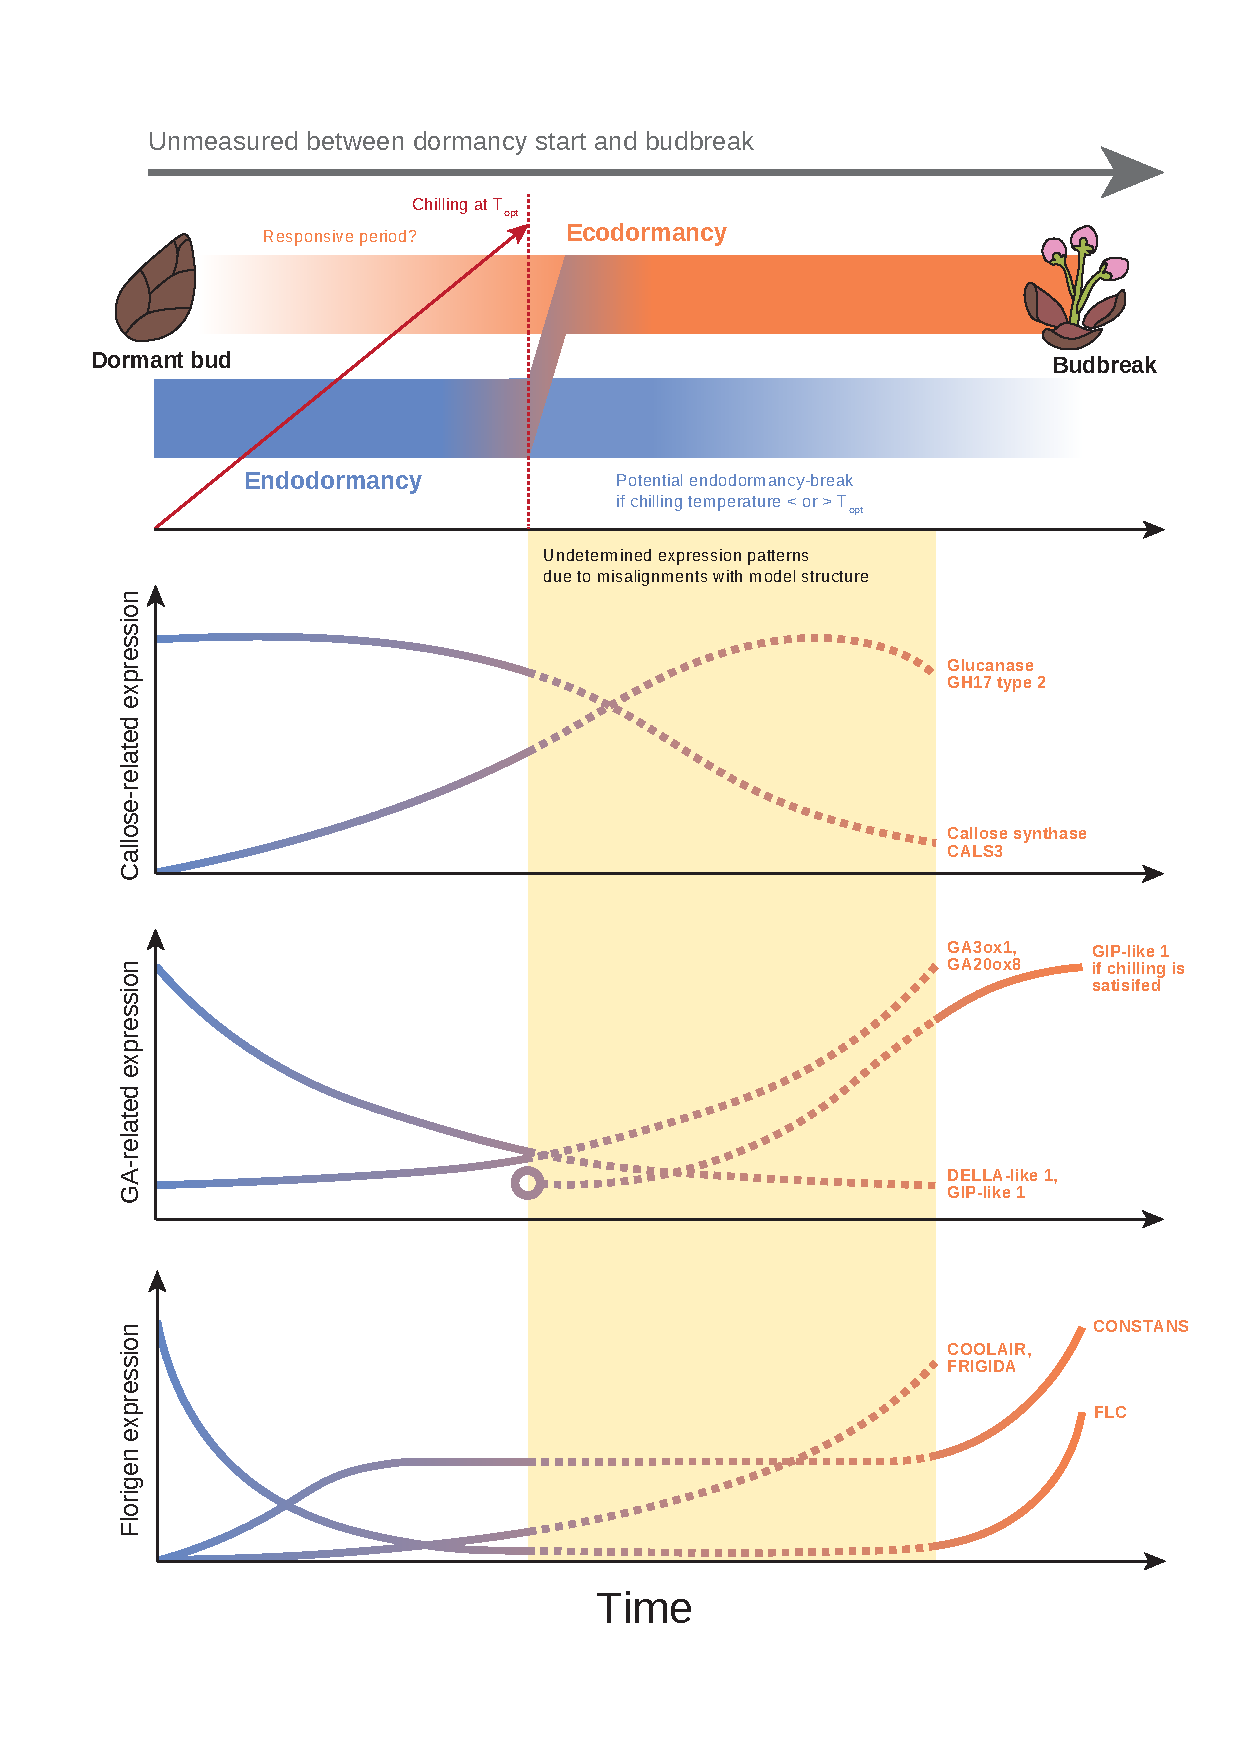
\includegraphics[width=0.7\textwidth]{..//figures/conceptModel/conceptModel_gradient.pdf}
\caption{Aligning phenological models and molecular findings. Current phenological models of budbreak (top panel) assume two underlying states that lead to the observed process of budbreak: (1) endodormancy during which plants accumulate sufficient chilling to break endodormancy and transition to (2) ecodormancy, a period during which plants accumulate sufficient `forcing' (warm temperatures) to break bud (flower or leaf). Over 30 variants of this model exist, including those where the phases are sequential (darker shading) or occur in parallel (dark and light shading). Molecular work suggests callose (second panel), alongside gibberellic acid (GA, third panel) and circadian clock-related genes (fourth panel) may all underlie these hypothesized phases.} 
\label{fig:modelsketch}
\end{figure}


\begin{figure}[h!] 
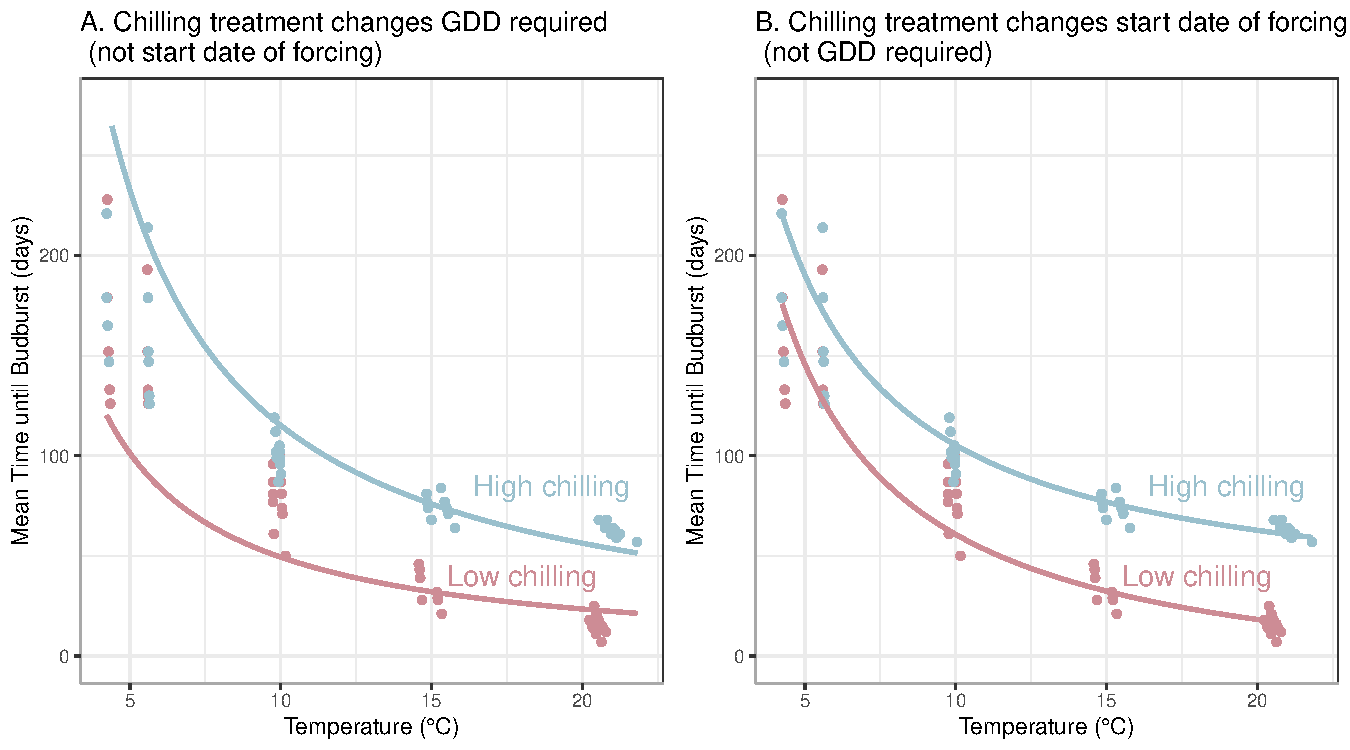
\includegraphics[width=0.99\textwidth]{..//figures/quickcompare.pdf}
\caption{Many experiments studying chilling alter `chilling' and `forcing' by varying the duration that cool temperatures are applied (`chilling') followed by different warm temperatures (`forcing'). Fitting simple linear models to these data (e.g., ANOVA models, with main effects of `chilling' and `forcing' treatments and their interaction---`chilling' $\times$ `forcing'---to find a sub-additive effect of the two) usually does not match the current biological understanding of chilling. Fitting models that match the proposed accumulation process is possible, however, as we show here using data from \citet{walde2022higher} for \emph{Quercus robur}, and considering two alternative biologies: (A) cool (`chilling') and warm treatments ($x$ axis) interact, such that longer cool temperatures mean more warm temperatures are required for leafout, versus (B) longer cool temperatures change the start date of the accumulation of warm (`forcing') temperatures (also known as endodormancy break). } %This approach could help better link statistical models with the current biological understanding of chilling, but are still limited in that they cannot discern when and at what temperatures plants accumulate chilling and forcing.
\label{fig:multimodelexps}
\end{figure}
% Data from Walde: https://datadryad.org/dataset/doi:10.5061/dryad.x95x69pnp

\end{document}



